\section{Von Klitzing Constant}

The Hall resistance $\rho_{\text{xy}}$ forms plateaus at \begin{align}
    \rho_{xy} = \frac{h}{\nu e^2} =: \frac{R_\text K}{\nu} \end{align} with the elementary charge $e$ and the planck constant $h$. 
The filling factor $\nu \in \mathbb N$ describes the number of occupied Landau levels.
The goal of this section is to determine the von Klitzing constant $R_\text{K}$.
Before reading off the plateaus, two errors have to be taken into account: the time delay and the different scales of the lock in the amplifiers.
To account for the time delay caused by integration and possibly some additional internal delay of the lock-in amplifiers, the three voltages given by the lock-in amplifiers are shifted back in time.
Since the magnetic field B is ramped up and down between $0\,\text{T}$ and $9\,\text{T}$, the constant time shift can be chosen so that both graphs match.
To compensate for the different scales $\alpha_i$, the lock in amplifiers $1$ and $2$ measuring $U_\text{xy}$ and $U_\text I$ are swapped and the measurement is repeated at $1.4\,K$.
If $U$ and $I$ are the real values, then 
\begin{align}
    R_{\text K,1} = \frac{U_{\text{xy}, 1}}{I_2} = \frac{\alpha_1 U}{\alpha_2 I}\\ R_{\text K,2} = \frac{U_{\text{xy}, 2}}{I_1} = \frac{\alpha_2 U}{\alpha_1 I}
\end{align} 
One finds the correction factor 
\begin{align}
    \alpha = \frac{\alpha_1}{\alpha_2} = \sqrt{\frac{U_{\text{xy},1}I_2}{U_{\text{xy}, 2}I_1}}. 
\end{align}
All further calculations are corrected for the time delay and the different scales.
Only $\rho_{\text{xy}}$ is corrected with the factor $\alpha$, since no additional measurement with swapped lock-in amplifiers was performed.
In principle, $\rho_{\text{xx}}$ could be corrected in the same way.
The longitudinal and transverse resistance for $T=1.4\,\text{K}$ and a gate voltage of $U_\text{gate}=-0.25\,\text{V}$ is shown in fig. \ref{fig:KlitzingBeispielBild} \begin{figure}[h] \centering 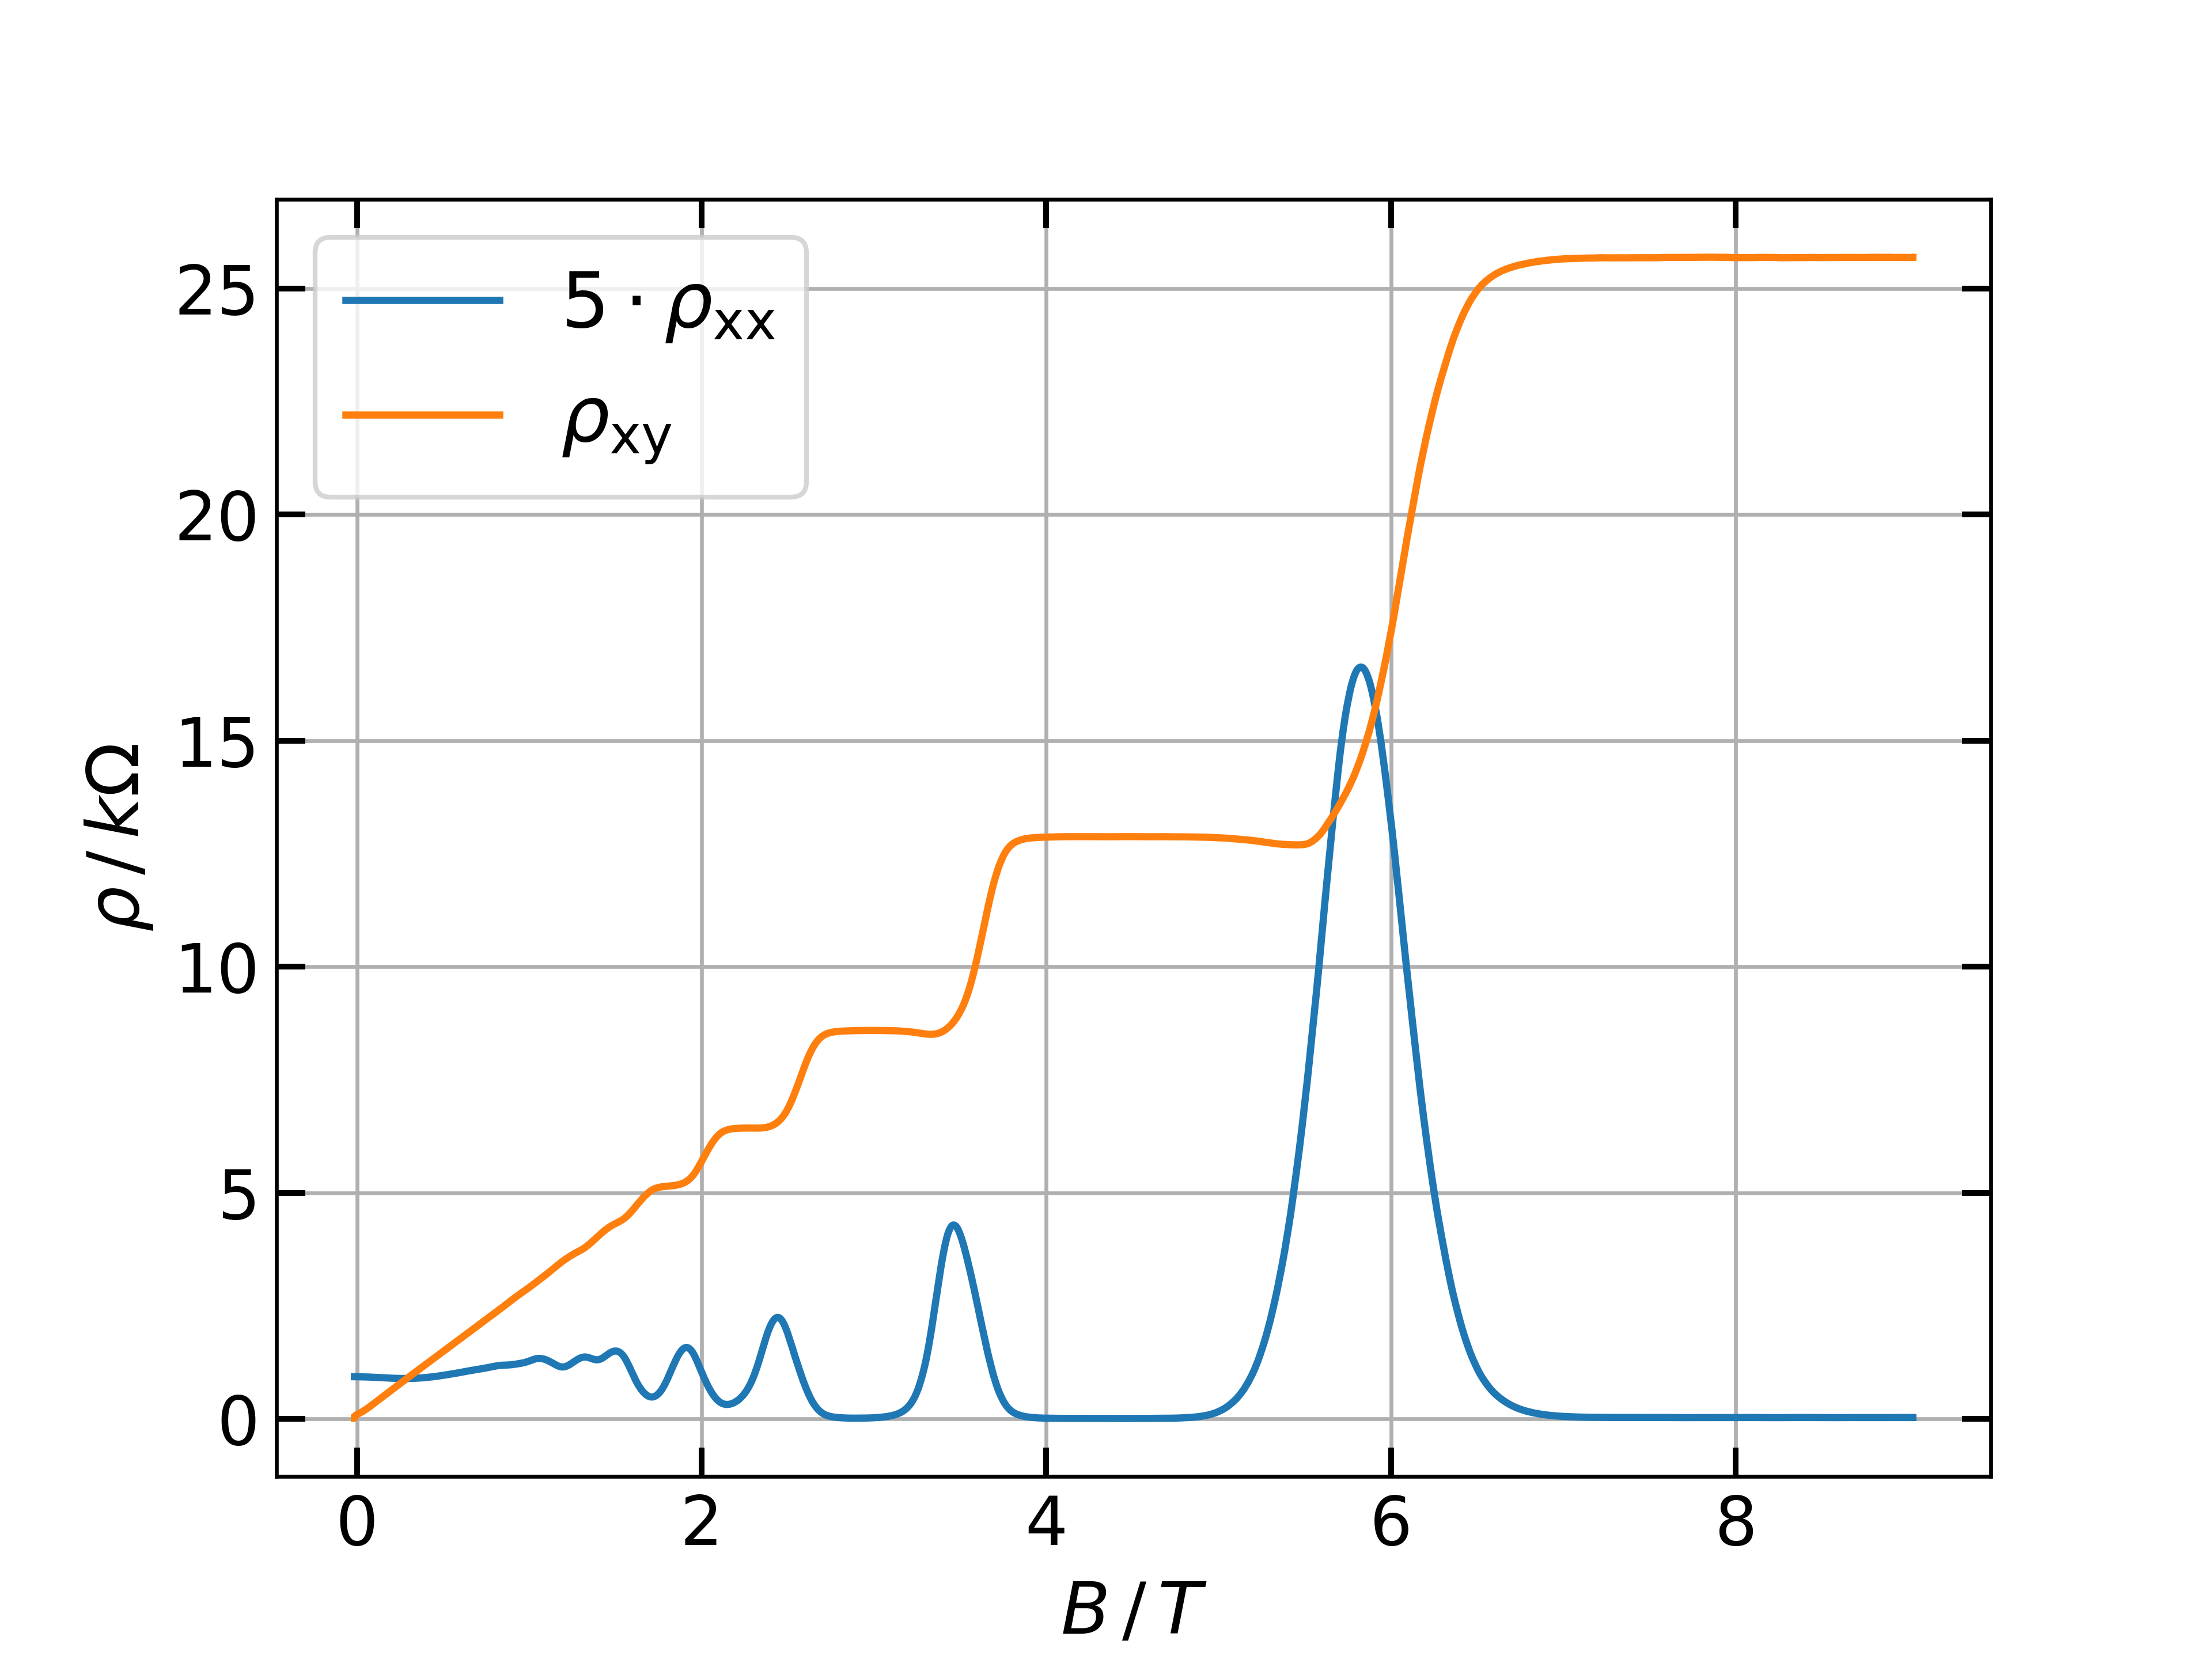
\includegraphics[width=0.45\textwidth]{../Images/BeispielBildVomAnfang.png}
    \caption{ Longitudinal and transverse resistivity for $T=1.4\,\text{K}$ and a gate voltage of $U_\text{gate}=-0.25\,\text{V}$.
        Plateaus in the transverse resistivity and oscillating peaks in the longitudinal resistivity are clearly visible.
        $\rho_\text{xx}$ is scaled by a factor of 5.
        }
    \label{fig:KlitzingBeispielBild} 
\end{figure}
\\
To obtain $R_\text K$, the average of the resistivities of the plateaus are taken.
The transverse resistivity $\rho_{\text{xy}}$ of the plateaus and the resulting $R_\text{K}$ are listed in tab. \ref{tab:plateau_values} and tab. \ref{tab:Klitzing} respectively.
The error is obtained by propagating the accuracy of the lock in amplifiers.
\begin{table}[!ht]
    \centering
    \begin{tabular}{c|c c c c}
        $\nu$  & $4.2\,\text{K}$        & $3.0\,\text{K}$        & $2.1\,\text{K}$        & $1.4\,\text{K}$        \\ \hline
        1      & $\csname PlateauNr14.2K\endcsname$  & $\csname PlateauNr13K\endcsname$  & $\csname PlateauNr12.1K\endcsname$  & $\csname PlateauNr11.4K\endcsname$  \\ 
        2      & $\csname PlateauNr24.2K\endcsname$  & $\csname PlateauNr23K\endcsname$  & $\csname PlateauNr22.1K\endcsname$  & $\csname PlateauNr21.4K\endcsname$  \\ 
        3      & $\csname PlateauNr34.2K\endcsname$  & $\csname PlateauNr33K\endcsname$  & $\csname PlateauNr32.1K\endcsname$  & $\csname PlateauNr31.4K\endcsname$  \\ 
        4      & $\csname PlateauNr44.2K\endcsname$  & $\csname PlateauNr43K\endcsname$  & $\csname PlateauNr42.1K\endcsname$  & $\csname PlateauNr41.4K\endcsname$  \\ 
        5      & $\csname PlateauNr54.2K\endcsname$  & $\csname PlateauNr53K\endcsname$  & $\csname PlateauNr52.1K\endcsname$  & $\csname PlateauNr51.4K\endcsname$  \\ 
    \end{tabular}
    \caption{Plateaus in Hall resistivity for different temperatures and filling factors in $\text{k}\Omega$.
    The error is $1.4\%$.
    }
    \label{tab:plateau_values}
\end{table}
\begin{table}[h!]
    \centering
    \begin{tabular}{c|c c c c}
        $\nu$  & $4.2\,\text{K}$        & $3.0\,\text{K}$        & $2.1\,\text{K}$        & $1.4\,\text{K}$        \\ \hline
        1      & $\csname PlateauMalNuNr14.2K\endcsname$  & $\csname PlateauMalNuNr13K\endcsname$  & $\csname PlateauMalNuNr12.1K\endcsname$  & $\csname PlateauMalNuNr11.4K\endcsname$  \\ 
        2      & $\csname PlateauMalNuNr24.2K\endcsname$  & $\csname PlateauMalNuNr23K\endcsname$  & $\csname PlateauMalNuNr22.1K\endcsname$  & $\csname PlateauMalNuNr21.4K\endcsname$  \\ 
        3      & $\csname PlateauMalNuNr34.2K\endcsname$  & $\csname PlateauMalNuNr33K\endcsname$  & $\csname PlateauMalNuNr32.1K\endcsname$  & $\csname PlateauMalNuNr31.4K\endcsname$  \\ 
        4      & $\csname PlateauMalNuNr44.2K\endcsname$  & $\csname PlateauMalNuNr43K\endcsname$  & $\csname PlateauMalNuNr42.1K\endcsname$  & $\csname PlateauMalNuNr41.4K\endcsname$  \\ 
        5      & $\csname PlateauMalNuNr54.2K\endcsname$  & $\csname PlateauMalNuNr53K\endcsname$  & $\csname PlateauMalNuNr52.1K\endcsname$  & $\csname PlateauMalNuNr51.4K\endcsname$  \\ 
    \end{tabular}
    \caption{$R_\text K$ for different temperatures and filling factors in $\text{k}\Omega$.
    The error is $1.4\%$.
    }
    \label{tab:Klitzing}
\end{table}
\begin{table}[!ht]
    \centering
    \begin{tabular}{c|c}
        $T\,/\,\text{K}$  & $R_\text{K} \, / \, \text{k}\Omega$  \\ \hline
        4.2      & $\csname Klitzing4.2K\endcsname$  \\ 
        3.0      & $\csname Klitzing3K\endcsname$   \\ 
        2.1      & $\csname Klitzing2.1K\endcsname$   \\ 
        1.4      & $\csname Klitzing1.4K\endcsname$  \\ 
    \end{tabular}
    \caption{Von Klitzing constant $R_\text K$ measured at different temperatures.
    }
    \label{tab:Klitzing2}
\end{table}
To determine the von Klizing constant, measured at different temperatures, the average value for different $\nu$ is taken.
The results are shown in tab \ref{tab:Klitzing2}.
The results match the exact defined value of $R_\text{K, exact} = 2.581280...$ \cite{klitzing}. 




